% Created 2021-04-11 Sun 22:13
% Intended LaTeX compiler: pdflatex
\documentclass[presentation]{beamer}
\usepackage[utf8]{inputenc}
\usepackage[T1]{fontenc}
\usepackage{graphicx}
\usepackage{grffile}
\usepackage{longtable}
\usepackage{wrapfig}
\usepackage{rotating}
\usepackage[normalem]{ulem}
\usepackage{amsmath}
\usepackage{textcomp}
\usepackage{amssymb}
\usepackage{capt-of}
\usepackage{hyperref}
\usetheme{Warsaw}
\hypersetup{
colorlinks=true,%
urlcolor=blue,%
linkcolor=blue%
}
\usepackage[gen]{eurosym}    % For € symbol
\usepackage{wasysym}         % For smileys
\usepackage{bclogo}          % For bcattention & bccrayon signs
\usepackage{fontawesome}     % For pretty UTF-8 emojis \faWarning \faExclamationTriangle
\usepackage{tikz}            % For drawings
\usetikzlibrary{arrows.meta} % For arrow heads
\usetikzlibrary{shadows}
\usepackage{tikzsymbols}     % For Sticky man
\usepackage{listings}        % To insert Java code listing
\definecolor{dkgreen}{rgb}{0,0.6,0}  %% Colors for the Java listings
\definecolor{gray}{rgb}{0.5,0.5,0.5}
\definecolor{mauve}{rgb}{0.58,0,0.82}
\lstset{frame=none,          % For Java listings
language=C,
aboveskip=1mm,
belowskip=1mm,
showstringspaces=false,
columns=flexible,
basicstyle={\scriptsize \ttfamily},
numbers=left,
numberstyle=\scriptsize\color{gray},
keywordstyle=\color{blue},
commentstyle=\color{dkgreen},
stringstyle=\color{mauve},
breaklines=true,
breakatwhitespace=true,
tabsize=2
}
\setbeamercolor{normal text}{fg=white,bg=black!90}
\setbeamercolor{structure}{fg=white} %% TODO Problem with "description" env!
\setbeamercolor{alerted text}{fg=red!85!black}
\setbeamercolor{item projected}{use=item,fg=black,bg=item.fg!35}
\setbeamercolor*{palette primary}{use=structure,fg=structure.fg}
\setbeamercolor*{palette secondary}{use=structure,fg=structure.fg!95!black}
\setbeamercolor*{palette tertiary}{use=structure,fg=structure.fg!90!black}
\setbeamercolor*{palette quaternary}{use=structure,fg=structure.fg!95!black,bg=black!80}
\setbeamercolor*{framesubtitle}{fg=white}
\setbeamercolor*{block title}{parent=structure,bg=black!60}
\setbeamercolor*{block body}{fg=black,bg=black!10}
\setbeamercolor*{block title alerted}{parent=alerted text,bg=black!15}
\setbeamercolor*{block title example}{parent=example text,bg=black!15}
\setbeamertemplate{navigation symbols}{}
\setbeamertemplate{headline}{}
\addtobeamertemplate{navigation symbols}{}{%
\usebeamerfont{footline}%
\usebeamercolor[fg]{footline}%
\hspace{1em}%
\insertframenumber{}/\inserttotalframenumber{}
}
\AtBeginSection[]
{
\begin{frame}<beamer>
%\frametitle{Outline for section \thesection}
\tableofcontents[currentsection]
\end{frame}
}
\newcommand{\myarrow}[6]{ % size / src / linestyle / text / arrowhead / dest
\begin{tikzpicture}[baseline=-0.5ex]{
\node[inner sep=0](@1) at (0,0) {#2};
\node[inner sep=0](@2) at (#1,0) {#6};
\draw [#3,arrows={#5},shorten >= 2pt,shorten <= 2pt] (@1) -- (@2) node[pos=.5,above,inner sep=1pt] { #4 };}
\end{tikzpicture}\xspace
}
\def\up#1{$^\text{#1}$}
\newcommand{\FrFlag}{\includegraphics[height=1.5em]{../images/UML/Lecture1/flag_france.png}}
\newcommand{\LOTRing}{\includegraphics[height=1.5em]{../images/UML/Lecture1/LOTR_1Ring.png}}
\usetheme{default}
\author{Guillaume MULLER}
\date{\today}
\title{High Performance Programming -- SIMD -- Vector Processors}
\title[HPP -- SIMD -- Vector]{High Performance Programming\\SIMD -- Vector Processors}
\subtitle{FISE2-INFO2\\ {\tiny Based on "Lecture 14: SIMD Processing"\\Onur Mutlu, 2015}}
\hypersetup{
 pdfauthor={Guillaume MULLER},
 pdftitle={High Performance Programming -- SIMD -- Vector Processors},
 pdfkeywords={High-Performance Programming SIMD Vector-Processors},
 pdfsubject={High Performance Programming -- SIMD -- Vector Processors},
 pdfcreator={Emacs 26.3 (Org mode 9.4.5)}, 
 pdflang={English}}
\begin{document}

\maketitle

\section*{Intro}
\label{sec:org92cedf9}

\begin{frame}[label={sec:org59488e5}]{Readings}
\begin{block}{Paper1}
\begin{itemize}
\item \href{https://people.cs.umass.edu/\~emery/classes/cmpsci691st/readings/Arch/gpu.pdf}{\textsc{Lindholm} \emph{et al.}, "NVIDIA Tesla: A Unified Graphics and Computing Architecture", IEEE Micro 2008.}
\end{itemize}
\end{block}
\begin{block}{Paper2}
\begin{itemize}
\item \href{https://www.researchgate.net/publication/220422248\_A\_closer\_look\_at\_GPUs/link/550041e60cf204d683b34481/download}{\textsc{Fatahalian} and \textsc{Houston}, "A Closer Look at GPUs", CACM 2008.}
\end{itemize}
\end{block}
\end{frame}


\begin{frame}[label={sec:org38bb992}]{Reminder Intel Architecture}
\begin{center}
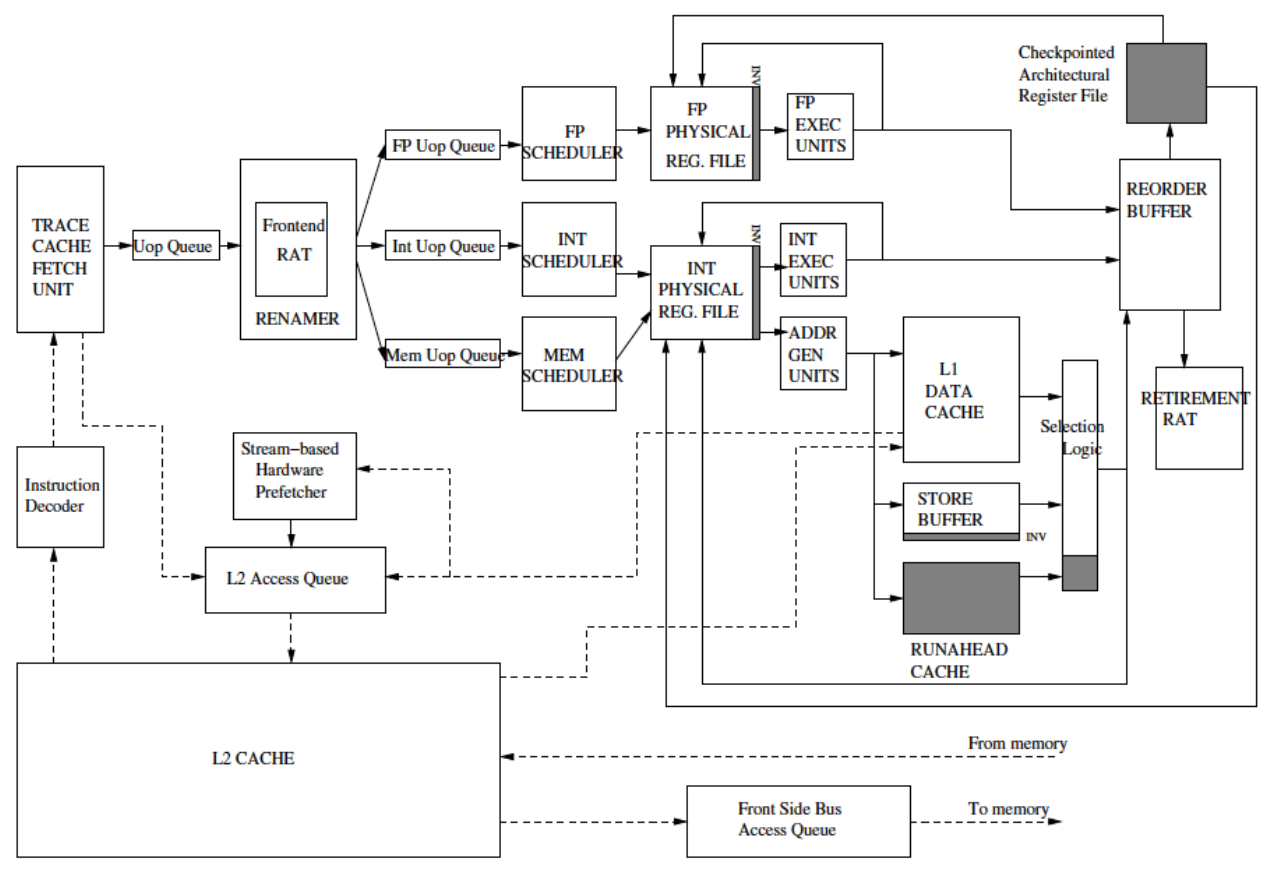
\includegraphics[width=.9\linewidth]{./images/slides_SIMD_08_small.png}
\end{center}
\begin{block}{Reference}
\begin{itemize}
\item \small \href{https://users.ece.cmu.edu/\~omutlu/pub/mutlu\_hpca03.pdf}{Mutlu \emph{et al.}, Runhead Execution, 2003}
\end{itemize}
\end{block}
\end{frame}


\begin{frame}[label={sec:orgc46e959}]{Reminder Alpha Architecture}
\begin{center}
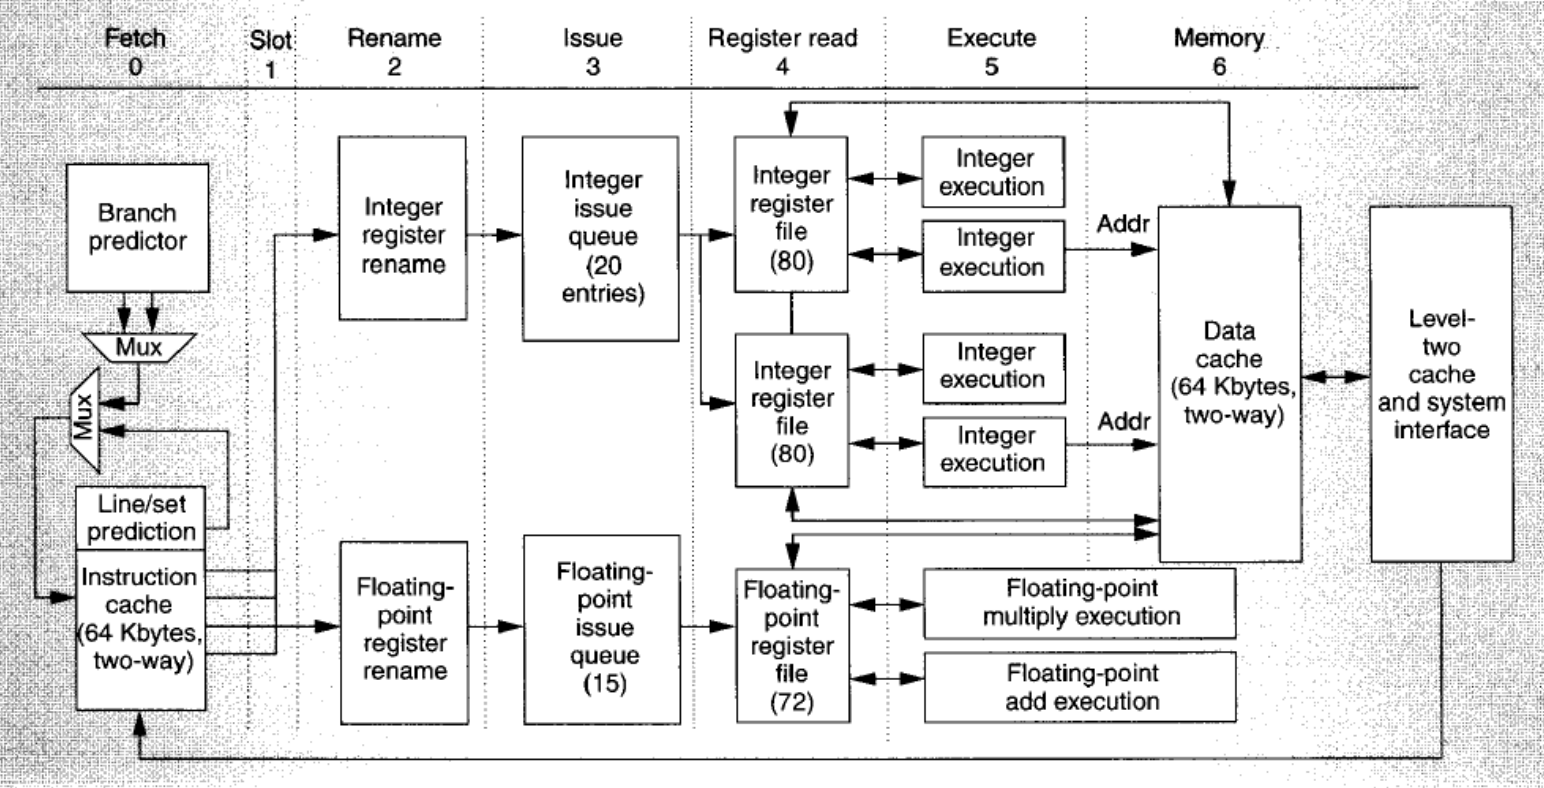
\includegraphics[width=.9\linewidth]{./images/slides_SIMD_09_small.png}
\end{center}
\begin{block}{Reference}
\begin{itemize}
\item \small \href{https://www.cis.upenn.edu/\~milom/cis501-Fall09/papers/Alpha21264.pdf}{Kessler, "The Alpha 21264 Microprocessor", IEEE Micro, March-April 1999.}
\end{itemize}
\end{block}
\end{frame}


\begin{frame}[label={sec:org430c225}]{SIMD: Exploiting Regular (Data) Parallelism}
\begin{block}{\href{https://course.ece.cmu.edu/\~ece447/s13/lib/exe/fetch.php?media=01447203.pdf}{Flynn's Taxonomy of Computers} (\alert{1966})}
\begin{itemize}
\item SISD: Single Instruction operates on Single Data
\pause
\item \alert{SIMD}: Single Instruction operates on Multiple Data
\begin{itemize}
\item Array processor
\item Vector processor
\end{itemize}
\pause
\item MISD: Multiple Instructions operate on Single Data
\begin{itemize}
\item (rare)
\end{itemize}
\pause
\item MIMD: Multiple Instructions operate on Multiple Data
\begin{itemize}
\item Multi-Processor
\item Multi-Threaded
\end{itemize}
\end{itemize}
\end{block}
\end{frame}


\begin{frame}[label={sec:orgf718051}]{Data Parallelism}
\begin{block}{Concurrency Model}
\begin{itemize}
\item \alert{Same} operations \alert{different} pieces of data
\begin{itemize}
\item \alert{SIMD}
\item E.g. dot product of 2 vectors
\item Instruction (operation) level
\end{itemize}
\end{itemize}
\pause
\end{block}
\begin{block}{\(\neq\) Threads}
\begin{itemize}
\item "Control" parallelism
\end{itemize}
\pause
\end{block}
\begin{block}{\(\neq\) Data Flow}
\begin{itemize}
\item (pipelines, branch prediction\ldots{})
\item \(\neq\) operations in parallel
\end{itemize}
\end{block}
\end{frame}


\begin{frame}[label={sec:org53f5036}]{SIMD Parallelism}
\begin{block}{Parallelism in \alert{Time}}
\begin{itemize}
\item \alert{Array} processors
\begin{itemize}
\item 1 Instruction on multiple data
\item at the \alert{same time}
\item using \alert{different spaces}
\end{itemize}
\end{itemize}
\pause
\end{block}
\begin{block}{Parallelism in \alert{Space}}
\begin{itemize}
\item \alert{Vector} processor
\begin{itemize}
\item 1 Instruction on multiple data
\item using the \alert{same space}
\item in \alert{consecutive time steps}
\end{itemize}
\end{itemize}
\end{block}
\end{frame}


\begin{frame}[label={sec:org5d450e4},fragile]{Array vs. Vector Processors}
 \begin{columns}
\begin{column}{.22\columnwidth}
\begin{block}{Code}
\lstset{language=asm,label= ,caption= ,captionpos=b,numbers=none}
\begin{lstlisting}
LD VR <- A[3:0]
ADD VR <- VR, 1
MUL VR <- VR, 2
ST  A[3:0] <- VR
\end{lstlisting}
\pause
\end{block}
\end{column}
\begin{column}{.77\columnwidth}
\begin{block}{Execution}
\begin{center}
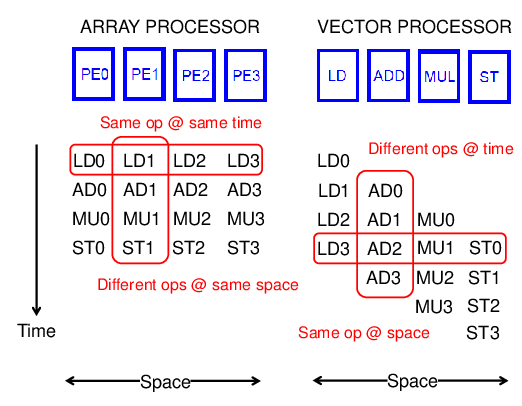
\includegraphics[width=.9\linewidth]{./images/slides_SIMD_19_small.png}
\end{center}
\end{block}
\end{column}
\end{columns}
\end{frame}



\begin{frame}[label={sec:org3403eb6}]{Array Processors}
\begin{block}{Array processors}
\begin{itemize}
\item Single operation on multiple (different) data elements
\end{itemize}
\pause
\end{block}

\begin{block}{}
\begin{center}
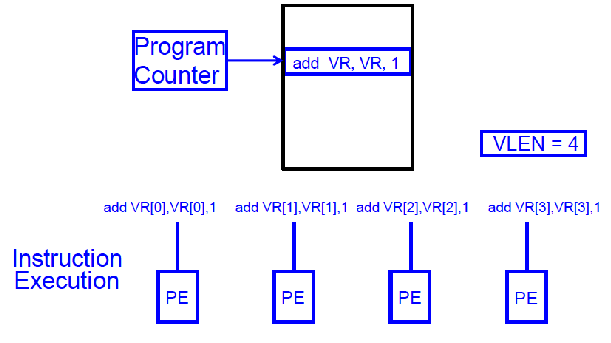
\includegraphics[width=.9\linewidth]{./images/slides_SIMD_21_small.png}
\end{center}
\end{block}
\end{frame}


\begin{frame}[label={sec:org75ee41c},fragile]{Vector Processors}
 \begin{block}{Vector processor}
\begin{itemize}
\item Operates on \emph{vectors} not \emph{scalars}
\item Scalar = Single value
\item Vector = 1D array of numbers
\begin{itemize}
\item Used in many scientific apps
\lstset{language=C,label= ,caption= ,captionpos=b,numbers=none}
\begin{lstlisting}
for (i = 0; i<=49; i++) {
  C[i] = (A[i] + B[i]) / 2
}
\end{lstlisting}
\end{itemize}
\end{itemize}
\pause
\end{block}
\begin{block}{Basic requirements}
\begin{itemize}
\item \alert{vector} registers
\item \alert{VLEN} (vector \emph{length} register)
\item \alert{VSTR} (vector \emph{stride} register)
\begin{itemize}
\item Stride: distance between two elements of a vector
\end{itemize}
\end{itemize}
\end{block}
\end{frame}


\begin{frame}[label={sec:org64290e2}]{Vector Processors}
\begin{block}{Vector Processors \& Pipelines}
\begin{itemize}
\item A vector instruction = each element in consecutive cycles
\item Vector functional units are \alert{pipelined}
\item Each pipeline stage operates on a different data element
\end{itemize}
\end{block}
\begin{block}{Vector Processors Advantages}
\begin{itemize}
\item \alert{No} intra-vector \alert{dependencies}
\begin{itemize}
\item \(\Rightarrow\) no hardware interlocking
\end{itemize}
\item \alert{No control flow} within a vector
\item Known stride
\begin{itemize}
\item \(\Rightarrow\) \alert{prefetching}
\end{itemize}
\end{itemize}
\end{block}
\end{frame}


\begin{frame}[label={sec:org30da707}]{Vector Processor Advantages}
\begin{block}{\alert{No dependencies} within a vector}
\begin{itemize}
\item Pipelining, parallelization work well
\item Can have very deep pipelines, no dependencies!
\end{itemize}
\end{block}

\begin{block}{Each instruction generates a lot of work}
\begin{itemize}
\item \alert{Reduces instruction fetch} bandwidth requirements
\end{itemize}
\end{block}

\begin{block}{Highly \alert{regular memory access pattern}}
\begin{itemize}
\item Can interleave vector data elements across multiple memory banks for higher memory bandwidth (to tolerate memory bank access latency)
\item Prefetching a vector is relatively easy
\end{itemize}
\end{block}

\begin{block}{No need to explicitly code loops}
\begin{itemize}
\item \alert{Fewer branches} in the instruction sequence
\end{itemize}
\end{block}
\end{frame}


\begin{frame}[label={sec:org97884dd}]{Vector Processor Disadvantages}
\begin{block}{Regular Parallelism}
\begin{itemize}
\item Works (only) if parallelism is regular (data/SIMD parallelism)
\begin{itemize}
\item = Vector operations
\end{itemize}
\item Very inefficient if parallelism is irregular
\begin{itemize}
\item How about searching for a key in a linked list?
\end{itemize}
\end{itemize}
\end{block}

\begin{block}{}
\href{https://courses.cs.washington.edu/courses/cse548/16wi/Fisher-VLIW.pdf}{\begin{quote}
"To program a vector machine, the compiler or hand coder must \alert{make the data structure in the code fit nearly exactly the regular structure built into the hardware}. That's hard to do in first place, and just as hard to change. One tweak, and the low-level code has to be \alert{rewritten} by a very smart and dedicated programmer who knows the hardware and often the subtelties of the application area."
\end{quote}} \hfill Fisher, 1983.
\end{block}
\end{frame}

\begin{frame}[label={sec:org201ba0c}]{Vector Processor Limitations}
\begin{block}{Memory}
\begin{itemize}
\item Memory (bandwidth) can become a bottleneck if:
\begin{enumerate}
\item compute/memory operation balance is not maintained
\item data is not mapped appropriately to memory banks
\end{enumerate}
\end{itemize}
\end{block}
\end{frame}


\section*{Vector processors in depth}
\label{sec:orga189fda}

\begin{frame}[label={sec:orga6e2540}]{Vector Registers}
\begin{block}{Vector control registers}
\begin{itemize}
\item \small VLEN, VSTR, VMASK
\end{itemize}
\end{block}

\begin{block}{Vector Registers}
\begin{itemize}
\item \small Each vector data register holds N \(\times\) M-bit values
\item \small Maximum VLEN can be N
\begin{itemize}
\item Maximum number of elements stored in a vector register
\end{itemize}
\end{itemize}
\end{block}

\begin{block}{Vector Mask Register (VMASK)}
\begin{itemize}
\item \small Indicates which elements of vector to operate on
\item \small Set by vector test instructions  \texttt{VMASK[i] = (Vk[i] == 0)}
\vspace*{-1em}
\end{itemize}

\begin{center}
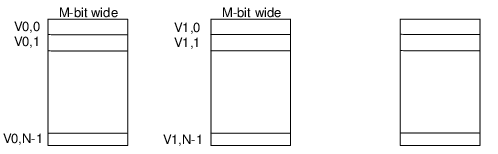
\includegraphics[width=.85\textwidth]{./images/slides_SIMD_28_small.png}
\end{center}
\end{block}
\end{frame}


\begin{frame}[label={sec:orgeeeb5e9},fragile]{Vector Functional Units}
 \begin{columns}
\begin{column}{.6\columnwidth}
\begin{block}{Pipelines}
\begin{itemize}
\item Vector elements are independent
\begin{itemize}
\item \(\Rightarrow\) \alert{Deep pipeline} control is easy
\end{itemize}
\item Using deep pipelines
\begin{itemize}
\item \(\Rightarrow\) \alert{Fast clock cycle}
\end{itemize}
\end{itemize}
\end{block}
\end{column}
\begin{column}{.39\columnwidth}
\begin{block}{Example}
\begin{itemize}
\item 6 stages multiply
\item \texttt{V1*V2 -> V3}
\end{itemize}
\begin{center}
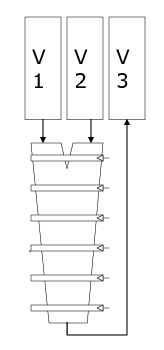
\includegraphics[width=.55\textwidth]{./images/slides_SIMD_29_small.png}
\end{center}
\end{block}
\end{column}
\end{columns}
\end{frame}


\begin{frame}[label={sec:orgef38a8a}]{Vector Machine Organization (CRAY-1)}
\begin{columns}
\begin{column}{.60\columnwidth}
\begin{block}{}
\begin{center}
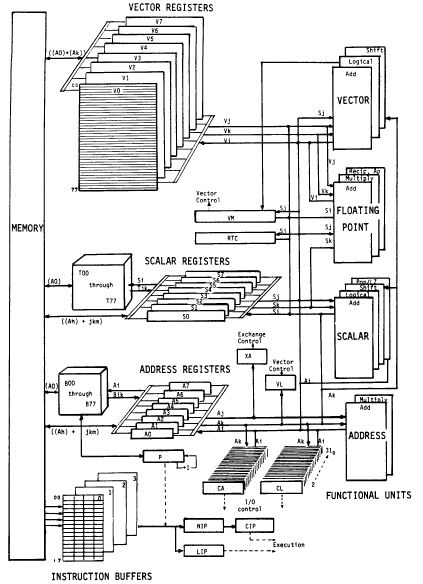
\includegraphics[width=.9\linewidth]{./images/slides_SIMD_30_small.png}
\end{center}
\end{block}
\end{column}

\begin{column}{.39\columnwidth}
\begin{block}{}
\begin{itemize}
\item \href{https://www.eecg.utoronto.ca/\~moshovos/ACA05/read/cray1.pdf}{CRAY-1}, 1978
\item scalar \& vector regs.
\item 8 \(\times\) 64 elts / reg
\item 64 bit / elt
\item 16 memory banks
\item 8 \(\times\) 64b scalar re.
\item 8 \(\times\) 24b addr. reg.
\end{itemize}
\end{block}
\end{column}
\end{columns}
\end{frame}


\begin{frame}[label={sec:org9090c74}]{Loading/Storing Vectors from/to Memory}
\begin{block}{}
\begin{itemize}
\item Requires loading/storing multiple elements
\item Elements separated by a \alert{constant} distance (stride)
\begin{itemize}
\item Assume stride = 1 for now
\end{itemize}
\item If we can start the load of one element per cycle
\begin{itemize}
\item Elements can be loaded in \alert{consecutive cycles}
\item \(\Rightarrow\) Can sustain a \alert{throughput of 1 elt/cycle}
\end{itemize}
\end{itemize}
\end{block}
\begin{block}{Question}
\begin{itemize}
\item How do we achieve this with a memory that takes more than 1 cycle to access?
\end{itemize}
\pause
\begin{itemize}
\item \(\Rightarrow\) \alert{Bank the memory}
\item \(\Rightarrow\) Interleave elements across banks
\end{itemize}
\end{block}
\end{frame}


\begin{frame}[label={sec:orgce8c22f}]{Memory Banking}
\begin{block}{Memory Banking}
\begin{itemize}
\item Memory is divided into \alert{independent banks}
\item But that \alert{share} address and data \alert{buses}
\item Can start and complete \alert{1 bank access/cycle}
\item Can sustain \alert{N parallel accesses} if all N go to different banks
\end{itemize}
\end{block}

\begin{block}{}
\begin{center}
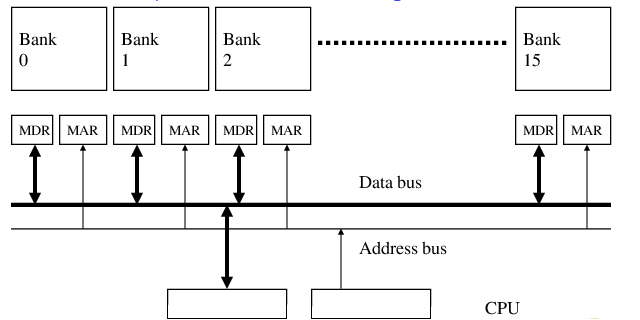
\includegraphics[width=.9\linewidth]{./images/slides_SIMD_32_small.png}
\end{center}
\end{block}
\end{frame}



\begin{frame}[label={sec:org5889203}]{Vector Memory System}
\begin{block}{Vector Memory System}
\begin{itemize}
\item Next address = Previous address + Stride
\item If
\begin{itemize}
\item stride = 1 \&
\item consecutive elements interleaved across banks \&
\item number of banks >= bank latency
\end{itemize}
\item then can sustain \alert{1 element/cycle}
\end{itemize}
\end{block}

\begin{block}{}
\begin{center}
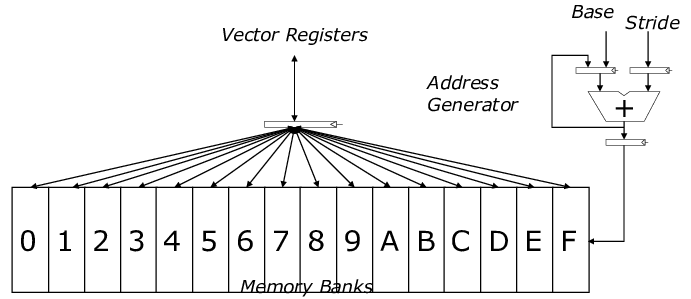
\includegraphics[width=.9\linewidth]{./images/slides_SIMD_33_small.png}
\end{center}
\end{block}
\end{frame}


\begin{frame}[label={sec:org22b6a6b},fragile]{Scalar Code Example}
 \begin{block}{C}
\lstset{language=C,label= ,caption= ,captionpos=b,numbers=none}
\begin{lstlisting}
for (i = 0; i<=49; i++) {
  C[i] = (A[i] + B[i]) / 2
}
\end{lstlisting}
\end{block}
\begin{block}{ASM (\emph{number = latency})}
\lstset{language=asm,label= ,caption= ,captionpos=b,numbers=none}
\begin{lstlisting}
MOVI R0 = 50               ; 1
MOVA R1 = A                ; 1
MOVA R2 = B                ; 1
MOVA R3 = C                ; 1
X: LD R4 = MEM[R1++]       ; 11 ; auto-inc
LD R5 = MEM[R2++]          ; 11
ADD R6 = R4 + R5           ; 4
SHFR R7 = R6 >> 1          ; 1
ST MEM[R3++] = R7          ; 11
DECBNZ --R0, X             ; 2 ; decr + brch non-0
\end{lstlisting}
\begin{itemize}
\item Number of \alert{instructions}: \alert{\(304\)}
\item Execution time: ??
\end{itemize}
\end{block}
\end{frame}


\begin{frame}[label={sec:org817acfd}]{Scalar Code Execution Time (In Order)}
\begin{block}{1 memory bank}
\begin{itemize}
\item First two loads in the loop cannot be pipelined
\begin{itemize}
\item \(\Rightarrow\) 2*11 cycles
\end{itemize}
\item \(4 + 50*40 =\) \alert{\(2004\)} cycles
\end{itemize}
\pause
\end{block}
\begin{block}{\alert{16} memory bank}
\begin{itemize}
\item First two loads in the loop can be pipelined
\item \(4 + 50*30 =\) \alert{\(1504\)} cycles
\end{itemize}
\pause
\end{block}
\begin{block}{Why \alert{16} banks?}
\pause
\begin{itemize}
\item 11 cycle memory access latency
\item 16 banks (>11 cycles)
\begin{itemize}
\item Enough to overlap enough mem. op. to cover mem. latency
\end{itemize}
\end{itemize}
\end{block}
\end{frame}


\begin{frame}[label={sec:org3c5e0d4},fragile]{Vectorizable Loops}
 \begin{block}{}
\begin{itemize}
\item Loop is \alert{vectorizable} if each iteration independent of others
\end{itemize}
\end{block}
\begin{block}{C}
\lstset{language=C,label= ,caption= ,captionpos=b,numbers=none}
\begin{lstlisting}
for (i = 0; i<=49; i++) {
  C[i] = (A[i] + B[i]) / 2
}
\end{lstlisting}
\end{block}
\begin{block}{Vectorized ASM (\emph{number = latency})}
\lstset{language=asm,label= ,caption= ,captionpos=b,numbers=none}
\begin{lstlisting}
MOVI VLEN = 50        ; 1
MOVI VSTR = 1         ; 1
VLD V0 = A            ; 11 + VLN-1
VLD V1 = B            ; 11 + VLN-1
VADD V2 = V0 + V1     ; 4  + VLN-1
VSHFR V3 = V2 >> 1    ; 1  + VLN-1
VST C = V3            ; 11 + VLN-1
\end{lstlisting}
\begin{itemize}
\item Number of \alert{instructions}: \alert{\(7\)}
\item Execution time: ??
\end{itemize}
\end{block}
\end{frame}


\begin{frame}[label={sec:org575ba1c}]{Vectorized Code Performance -- No Chaining}
\begin{block}{}
\begin{itemize}
\item Assume no chaining (no vector data forwarding)
\begin{itemize}
\item Output of a vector functional unit cannot be used as the direct input of another
\item The entire vector register needs to be ready before any element of it can be used as part of another operation
\end{itemize}
\item One memory port (one address generator)
\item 16 memory banks (word-interleaved)
\end{itemize}
\end{block}

\begin{block}{}
\begin{center}
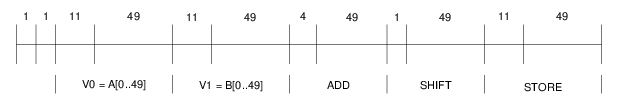
\includegraphics[width=.9\linewidth]{./images/slides_SIMD_37_small.png}
\end{center}

\begin{itemize}
\item \(2+2*(11+49)+4+49+1+49+11+49 =\) \alert{\(285\)} cycles
\end{itemize}
\end{block}
\end{frame}


\begin{frame}[label={sec:org99947d6}]{Vector Chaining}
\begin{block}{Vector chaining}
\begin{itemize}
\item Data forwarding from one vector functional unit to another
\end{itemize}
\end{block}

\begin{block}{}
\begin{center}
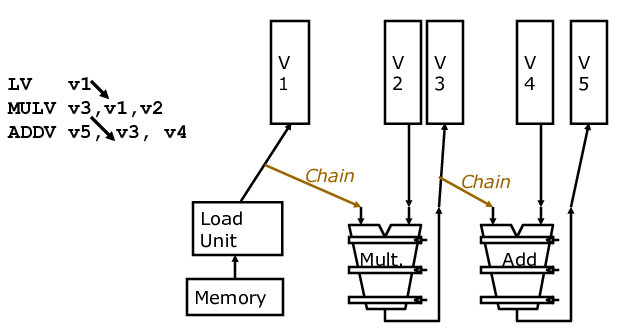
\includegraphics[width=.9\linewidth]{./images/slides_SIMD_38_small.png}
\end{center}
\end{block}
\end{frame}


\begin{frame}[label={sec:orge7f3ddf}]{Vectorized Code Performance -- With Chaining}
\begin{block}{}
\begin{center}
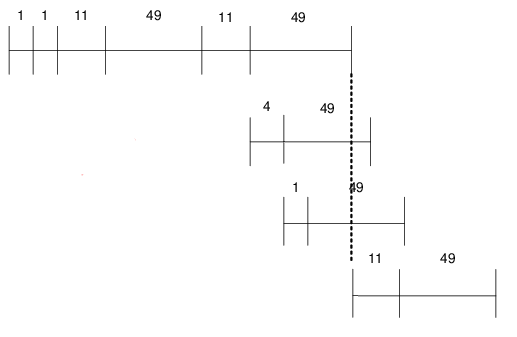
\includegraphics[width=.8\textwidth]{./images/slides_SIMD_39_small.png}
\end{center}
\end{block}

\begin{block}{}
\begin{itemize}
\item \(1+1+11+49+11+49+11+49=\) \alert{\(182\)} cycles
\end{itemize}
\pause
\begin{itemize}
\item \small 2 first VLD cannot be pipelined?
\item \small VLD \& VST cannot be pipelined?
\end{itemize}
\end{block}
\end{frame}


\begin{frame}[label={sec:org7c33384}]{Vectorized Code Performance -- Multiple Ports}
\begin{block}{}
\begin{center}
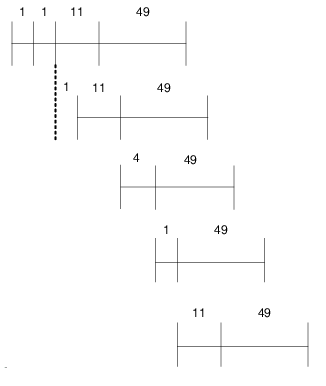
\includegraphics[width=.5\textwidth]{./images/slides_SIMD_40_small.png}
\end{center}
\end{block}

\begin{block}{}
\begin{itemize}
\item \(1+1+1+11+4+1+11+49 =\) \alert{\(79\)} cycles
\item \alert{\(19 \times\)} improvment!
\end{itemize}
\end{block}
\end{frame}


\begin{frame}[label={sec:orgb2b8259}]{Discussions}
\begin{block}{What if \#data elements > \#elements in a vector register?}
\pause
\begin{itemize}
\item Idea: Break loops
\begin{itemize}
\item Each iteration operates on \#elements vector register
\item E.g., 527 data elements, 64-element VREGs
\begin{itemize}
\item 8 iterations where VLEN = 64
\item 1 iteration where VLEN = 15 (need to change value of VLEN)
\end{itemize}
\end{itemize}
\end{itemize}
\pause
\begin{itemize}
\item Called \alert{"vector stripmining"}
\end{itemize}
\pause
\end{block}

\begin{block}{What if vector data is not stored in a strided fashion in memory?}
\pause

\begin{itemize}
\item Idea: Use indirection
\begin{itemize}
\item Combine/pack elements in vector registers
\end{itemize}
\item Called \alert{"scatter/gather operations"}
\end{itemize}
\end{block}
\end{frame}


\begin{frame}[label={sec:orgcb1d60b},fragile]{Gather/Scatter Operations}
 \begin{block}{Vectorize loops with indirect accesses}
\lstset{language=C,label= ,caption= ,captionpos=b,numbers=none}
\begin{lstlisting}
for (i=0; i<N; i++) {
  A[i] = B[i] + C[D[i]]
}
\end{lstlisting}
\end{block}
\begin{block}{Indexed load intruction (Gather)}
\lstset{language=asm,label= ,caption= ,captionpos=b,numbers=none}
\begin{lstlisting}
LV vD, rD         ; Load indices in D vector
LVI vC, rC, vD    ; Load indirect from rC base
LV vB, rB         ; Load B vector
ADDV.D vA,vB,vC   ; Do add
SV vA, rA         ; Store result
\end{lstlisting}
\end{block}
\end{frame}

\begin{frame}[label={sec:org25cf5f7}]{Gather/Scatter Operations}
\begin{block}{}
\begin{itemize}
\item Gather/scatter often implemented in hardware
\end{itemize}

\begin{itemize}
\item Vector load/store addresses = base register + index vector
\end{itemize}
\end{block}

\begin{block}{Example}
\begin{center}
\begin{tabular}{rrll}
Index Vector & Data Vector &  & Stored Vector\\
 & (to store) &  & (in memory)\\
0 & 3.14 & Base+0 & 3.14\\
2 & 6.5 & Base+1 & x\\
6 & 71.2 & Base+2 & 6.5\\
7 & 2.71 & Base+3 & x\\
 &  & Base+4 & x\\
 &  & Base+5 & x\\
 &  & Base+7 & 71.2\\
 &  & Base+7 & 2.71\\
\end{tabular}
\end{center}
\end{block}
\end{frame}


\begin{frame}[label={sec:orgbd38df5},fragile]{Conditional Operations in a Loop}
 \begin{block}{}
\begin{itemize}
\item What if some operations should not be executed on a vector?
\end{itemize}

\lstset{language=C,label= ,caption= ,captionpos=b,numbers=none}
\begin{lstlisting}
loop: if (a[i] != 0) {
   b[i] = a[i]*b[i];
}
goto loop
\end{lstlisting}
\pause
\end{block}
\begin{block}{Masked Operations}
\begin{itemize}
\item VMASK register is a bit mask determining which data element should not be acted upon
\end{itemize}
\lstset{language=asm,label= ,caption= ,captionpos=b,numbers=none}
\begin{lstlisting}
VLD V0 = A
VLD V1 = B
VMASK = (V0 != 0)
VMUL V1 = V0 * V1
VST B = V1
\end{lstlisting}
\end{block}
\end{frame}


\begin{frame}[label={sec:org5b8f9fc},fragile]{Another Example with Masking}
 \begin{columns}
\begin{column}{.35\columnwidth}
\begin{block}{C Code}
\lstset{language=C,label= ,caption= ,captionpos=b,numbers=none}
\begin{lstlisting}
for (i = 0; i < 64; ++i) {
  if (a[i] >= b[i]) {
    c[i] = a[i];
  } else {
    c[i] = b[i];
  }
}
\end{lstlisting}
\pause
\end{block}
\end{column}
\begin{column}{.60\columnwidth}
\begin{block}{}
\small
\begin{center}
\begin{tabular}{rrr}
A & B & VMASK\\
1 & 2 & 0\\
2 & 2 & 1\\
3 & 2 & 1\\
4 & 10 & 0\\
-5 & -4 & 0\\
0 & -3 & 1\\
6 & 5 & 1\\
-7 & -8 & 1\\
\end{tabular}
\end{center}
\end{block}
\end{column}
\end{columns}

\begin{block}{}
\end{block}

\begin{columns}
\begin{column}{1\columnwidth}
\begin{block}{Steps to execute the loop in SIMD code}
\begin{enumerate}
\item \alert{Compare A, B to get VMASK}
\item Masked store of A into C
\item Complement VMASK
\item Masked store of B into C
\end{enumerate}
\end{block}
\end{column}
\end{columns}
\end{frame}


\begin{frame}[label={sec:orgd749335}]{Masked Vector Instructions}
\begin{columns}
\begin{column}{.49\columnwidth}
\begin{block}<1->{Simple Implementation}
\begin{itemize}
\item \small Do all computations
\item \small Prevent writing of output
\end{itemize}
\begin{center}
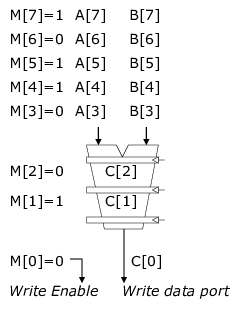
\includegraphics[width=.9\linewidth]{./images/slides_SIMD_46_small1.png}
\end{center}
\end{block}
\end{column}
\begin{column}[ignoreheading]{.49\columnwidth}
\begin{block}<2->{Density-Time Implementation}
\begin{itemize}
\item Scan mask vector
\item Only execute non-zero op
\end{itemize}
\begin{center}
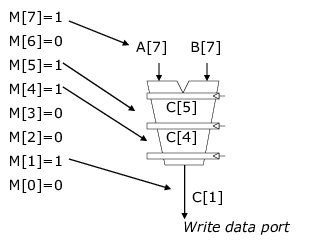
\includegraphics[width=.9\linewidth]{./images/slides_SIMD_46_small2.png}
\end{center}
\end{block}

\begin{block}<3->{Comparison}
\begin{itemize}
\item Which one is better?
\item Trade-Offs?
\end{itemize}
\end{block}
\end{column}
\end{columns}
\end{frame}



\begin{frame}[label={sec:org7cd59d6}]{Issues -- 1}
\begin{block}{Stride vs. Banking}
\begin{itemize}
\item To sustain 1 element/cycle throughput
\begin{itemize}
\item \#Banks \& Bank latency must be \alert{relatively prime}
\item Requires \alert{enough banks} to cover bank access latency
\end{itemize}
\item Storage of a matrix
\begin{itemize}
\item Row major vs. Column major (see next slide)
\item row \(\rightarrow\) column \(\Rightarrow\) \alert{change the stride}
\end{itemize}
\end{itemize}
\end{block}
\end{frame}


\begin{frame}[label={sec:orgf5a4537},plain]{Issues -- 2}
\begin{center}
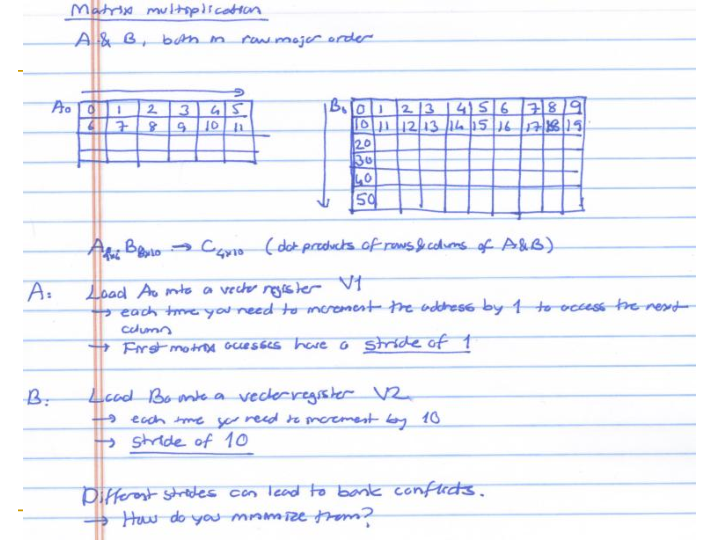
\includegraphics[width=.9\linewidth]{./images/slides_SIMD_48.png}
\end{center}
\end{frame}


\begin{frame}[label={sec:org0bbbed8}]{Minimizing Bank Conflicts}
\begin{block}{More banks}
\begin{itemize}
\item Adding Banks solves the problem, but \faDollar{}
\end{itemize}
\pause
\end{block}
\begin{block}{Better data layout to match the access pattern}
\begin{itemize}
\item Is this always possible?
\end{itemize}
\pause
\end{block}
\begin{block}{Better mapping of address to bank}
\begin{itemize}
\item E.g., \href{https://people.eecs.berkeley.edu/\~kubitron/courses/cs252-S12/handouts/papers/p74-rau.pdf}{randomized mapping}
\end{itemize}
\end{block}
\end{frame}


\begin{frame}[label={sec:org5e5ede6},fragile]{Automatic Code Vectorization}
 \begin{block}{}
\lstset{language=C,label= ,caption= ,captionpos=b,numbers=none}
\begin{lstlisting}
for (i = 0; i<=49; i++) {
  C[i] = (A[i] + B[i]) / 2
}
\end{lstlisting}
\end{block}

\begin{block}{}
\begin{center}
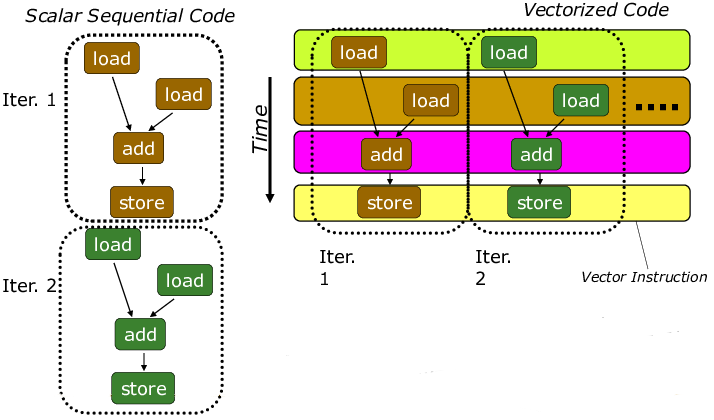
\includegraphics[width=.9\linewidth]{./images/slides_SIMD_55_small.png}
\end{center}
\end{block}
\end{frame}



\begin{frame}[label={sec:org825e974}]{Vector/SIMD Processing Summary}
\begin{block}{\alert{Data}-level parallelism}
\begin{itemize}
\item Same operation performed on many data elements
\item Improve performance, simplify design
\item No intra-vector dependencies
\end{itemize}
\end{block}
\begin{block}{\alert{Vectorizability} is the limit}
\begin{itemize}
\item Scalar operations limit vector machine performance
\item Remember \href{https://en.wikipedia.org/wiki/Amdahl\%27s\_law}{Amdahl's Law}
\end{itemize}

\begin{itemize}
\item CRAY-1 was the fastest \alert{scalar} machine at its time!
\end{itemize}
\end{block}
\begin{block}{\alert{Current} situation}
\begin{itemize}
\item Many existing ISAs include (vector-like) SIMD operations
\begin{itemize}
\item Intel MMX/SSE/AVX, ARM Advanced SIMD \ldots{}
\end{itemize}
\end{itemize}
\end{block}
\end{frame}


\begin{frame}[label={sec:org57597cc}]{Vector Processors vs. Array Processors}
\begin{block}{\alert{"purist's"} distinction}
\begin{itemize}
\item Array vs. vector processor distinction is a "purist's" distinction
\end{itemize}
\end{block}

\begin{block}{\alert{Current} situation}
\begin{itemize}
\item Most "modern" SIMD processors are a combination of both
\begin{itemize}
\item They exploit data parallelism in both \alert{time} and \alert{space}
\item GPUs are a prime example
\end{itemize}
\end{itemize}
\end{block}
\end{frame}
\end{document}